\section{Reconstruction}

The aim of the LTCC is to differentiate between pions and kaons. The lighter pions leave a signal in the detector,
while the heavier kaons pass through the detector without leaving a signal. To accomplish this, it is necessary to
associate the hits in the detector with their corresponding tracks. On average, the Cherenkov light from a charged
particle will hit between 1 and 3 adjacent PMTs. The task of the reconstruction program is therefore to (a) cluster
together the hits that belong to a single track and (b) provide the positional information needed to match the cluster
with the correct reconstructed track. The reconstruction program is implemented as an engine in the CLAS12 event
reconstruction framework~\cite{recon-nim}.

\subsection{Clustering Algorithm}

The Cherenkov cone associated with a charged particle is in all cases contained within a single sector of the LTCC.
This allows for a relatively straightforward clustering algorithm:

\begin{enumerate}
    \item Scan for the highest multiplicity hits, identified as the cluster center;
    \item Grow the cluster by adding all hits adjacent to the cluster center within this sector;
    \item Repeat the procedure until all hits have been assigned to a cluster.
\end{enumerate}

\subsection{Track Matching}

The \textit{true} cluster center can be defined as the position where the charged particle (and its Cherenkov cone)
crossed the elliptical mirror of the LTCC. Due to the geometry of the LTCC, this position does not uniquely correspond
to a single PMT, as the angle with which a particle crosses the elliptical mirrors depends on the particle momentum,
position, charge, and the torus magnetic field and polarity. The implies that, based solely on the LTCC hits, the
\textit{true} cluster position cannot be uniquely constrained. This is illustrated in \F{trackmatching}.

The track matching is performed in a stage of the reconstruction where the tracking information is available. In
order to perform the track matching, the estimated \textit{true} cluster position is recalculated for each track,
leveraging the Monte Carlo simulation of the LTCC to correctly associate a tentative \textit{true} cluster position
with the measured hits. The track that passes the closest to the tentative \textit{true} cluster position is then
chosen as the true match for this cluster.

\begin{figure}
  \centering
  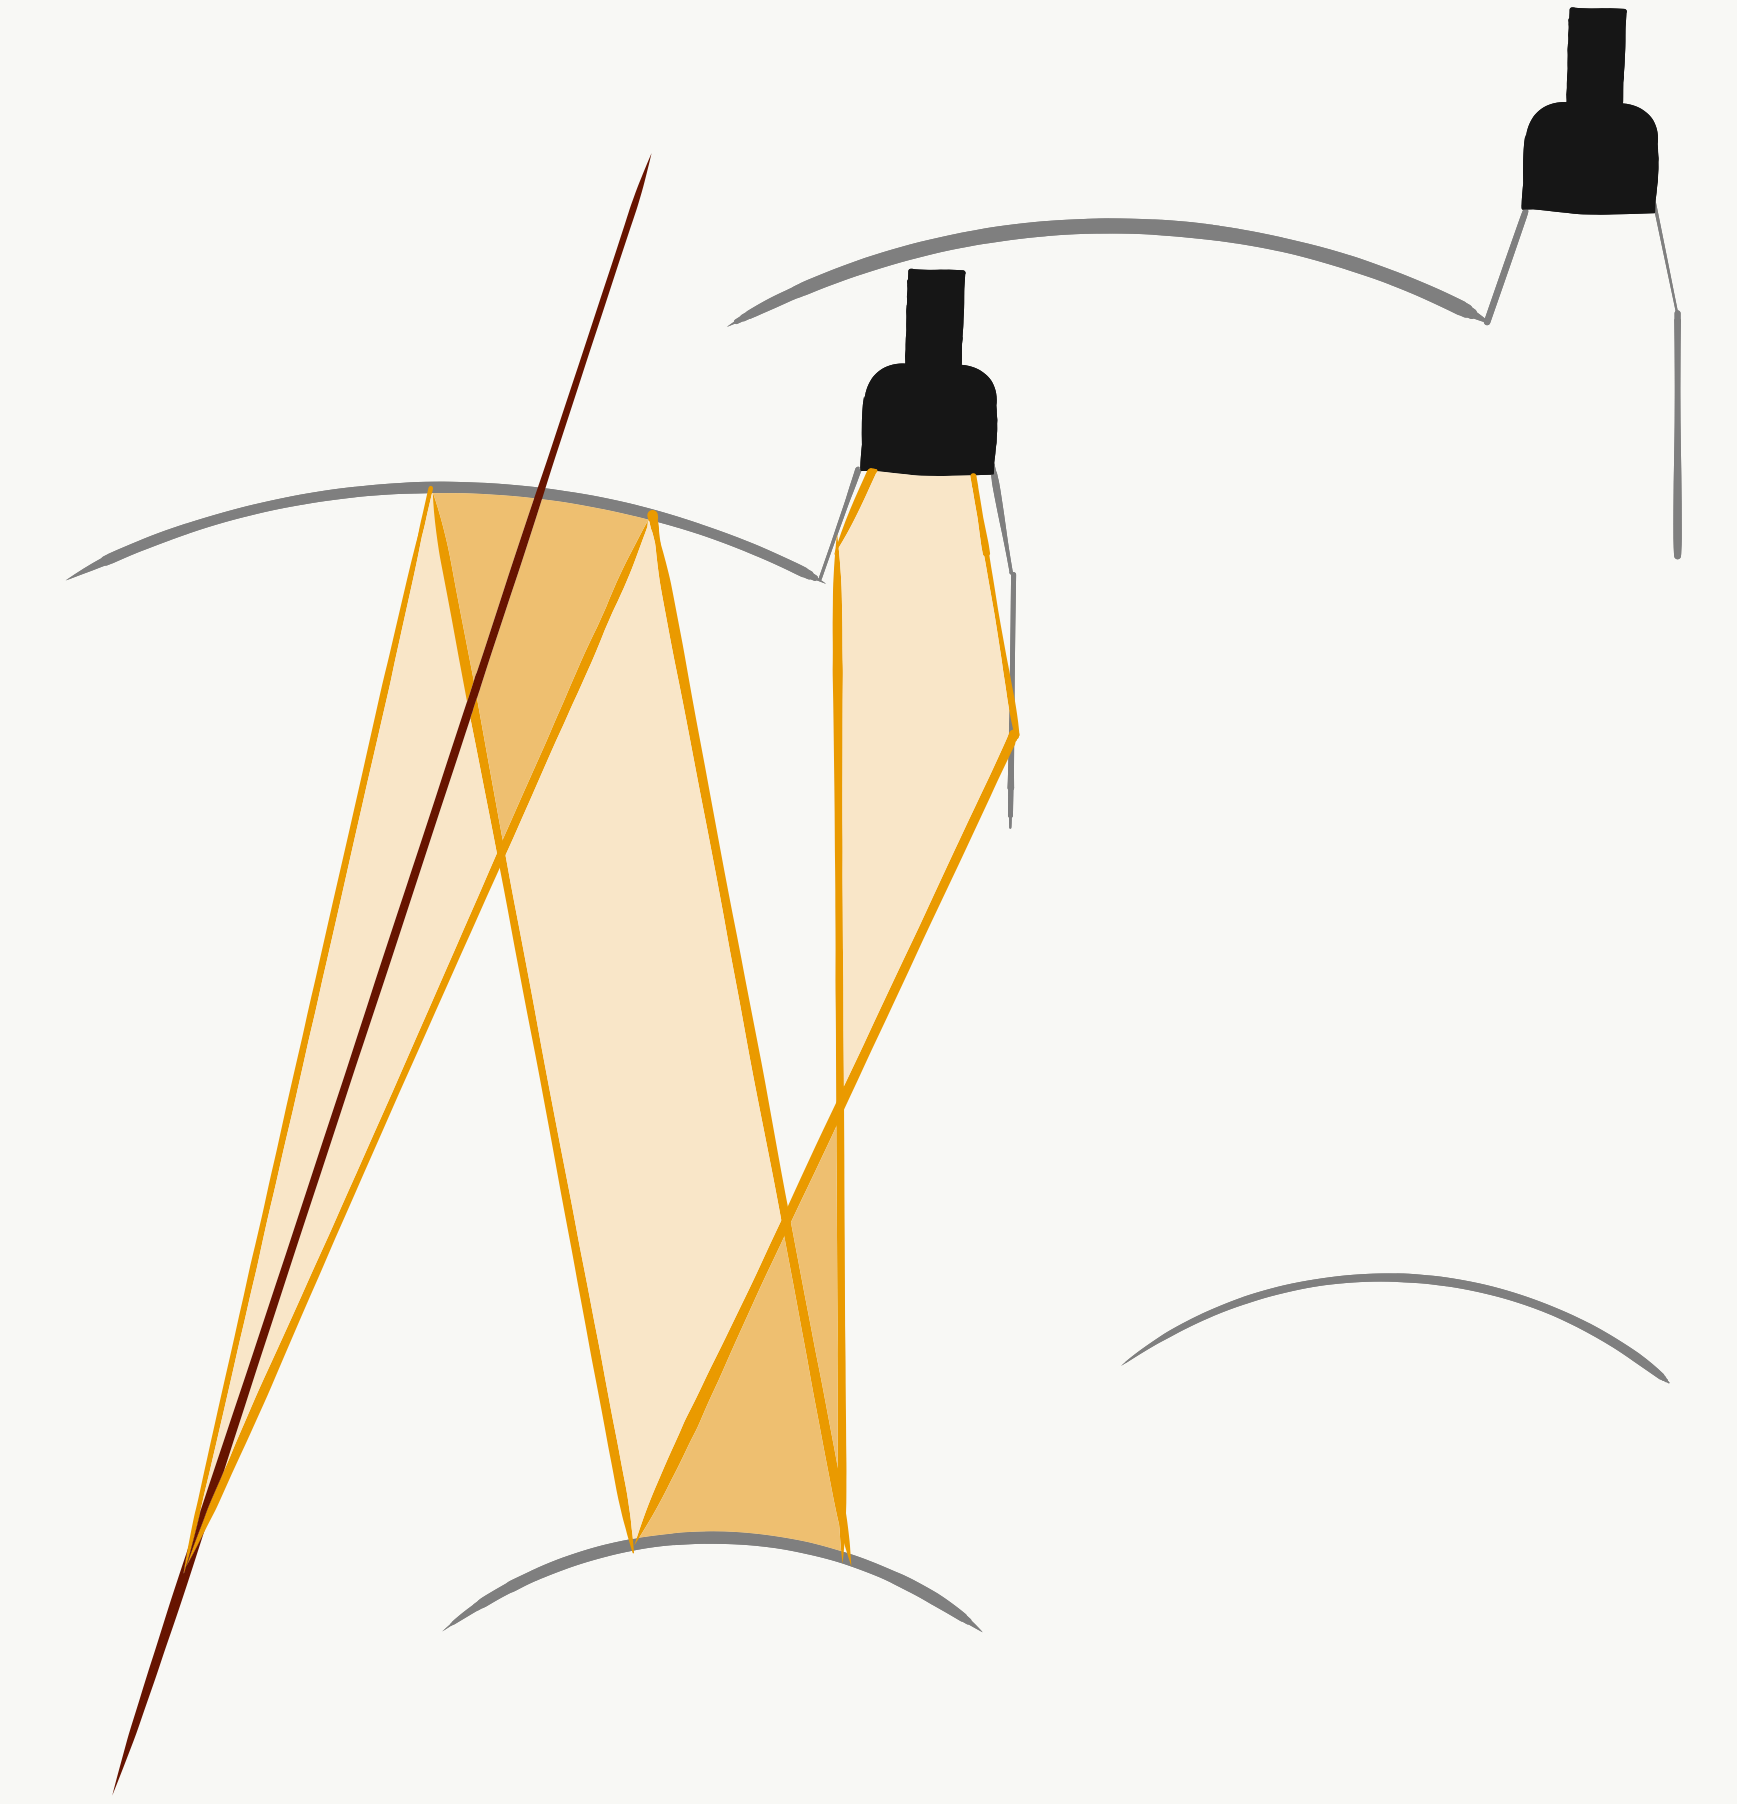
\includegraphics[width=0.99\columnwidth, keepaspectratio]{img/LTCC-event-1.png}
  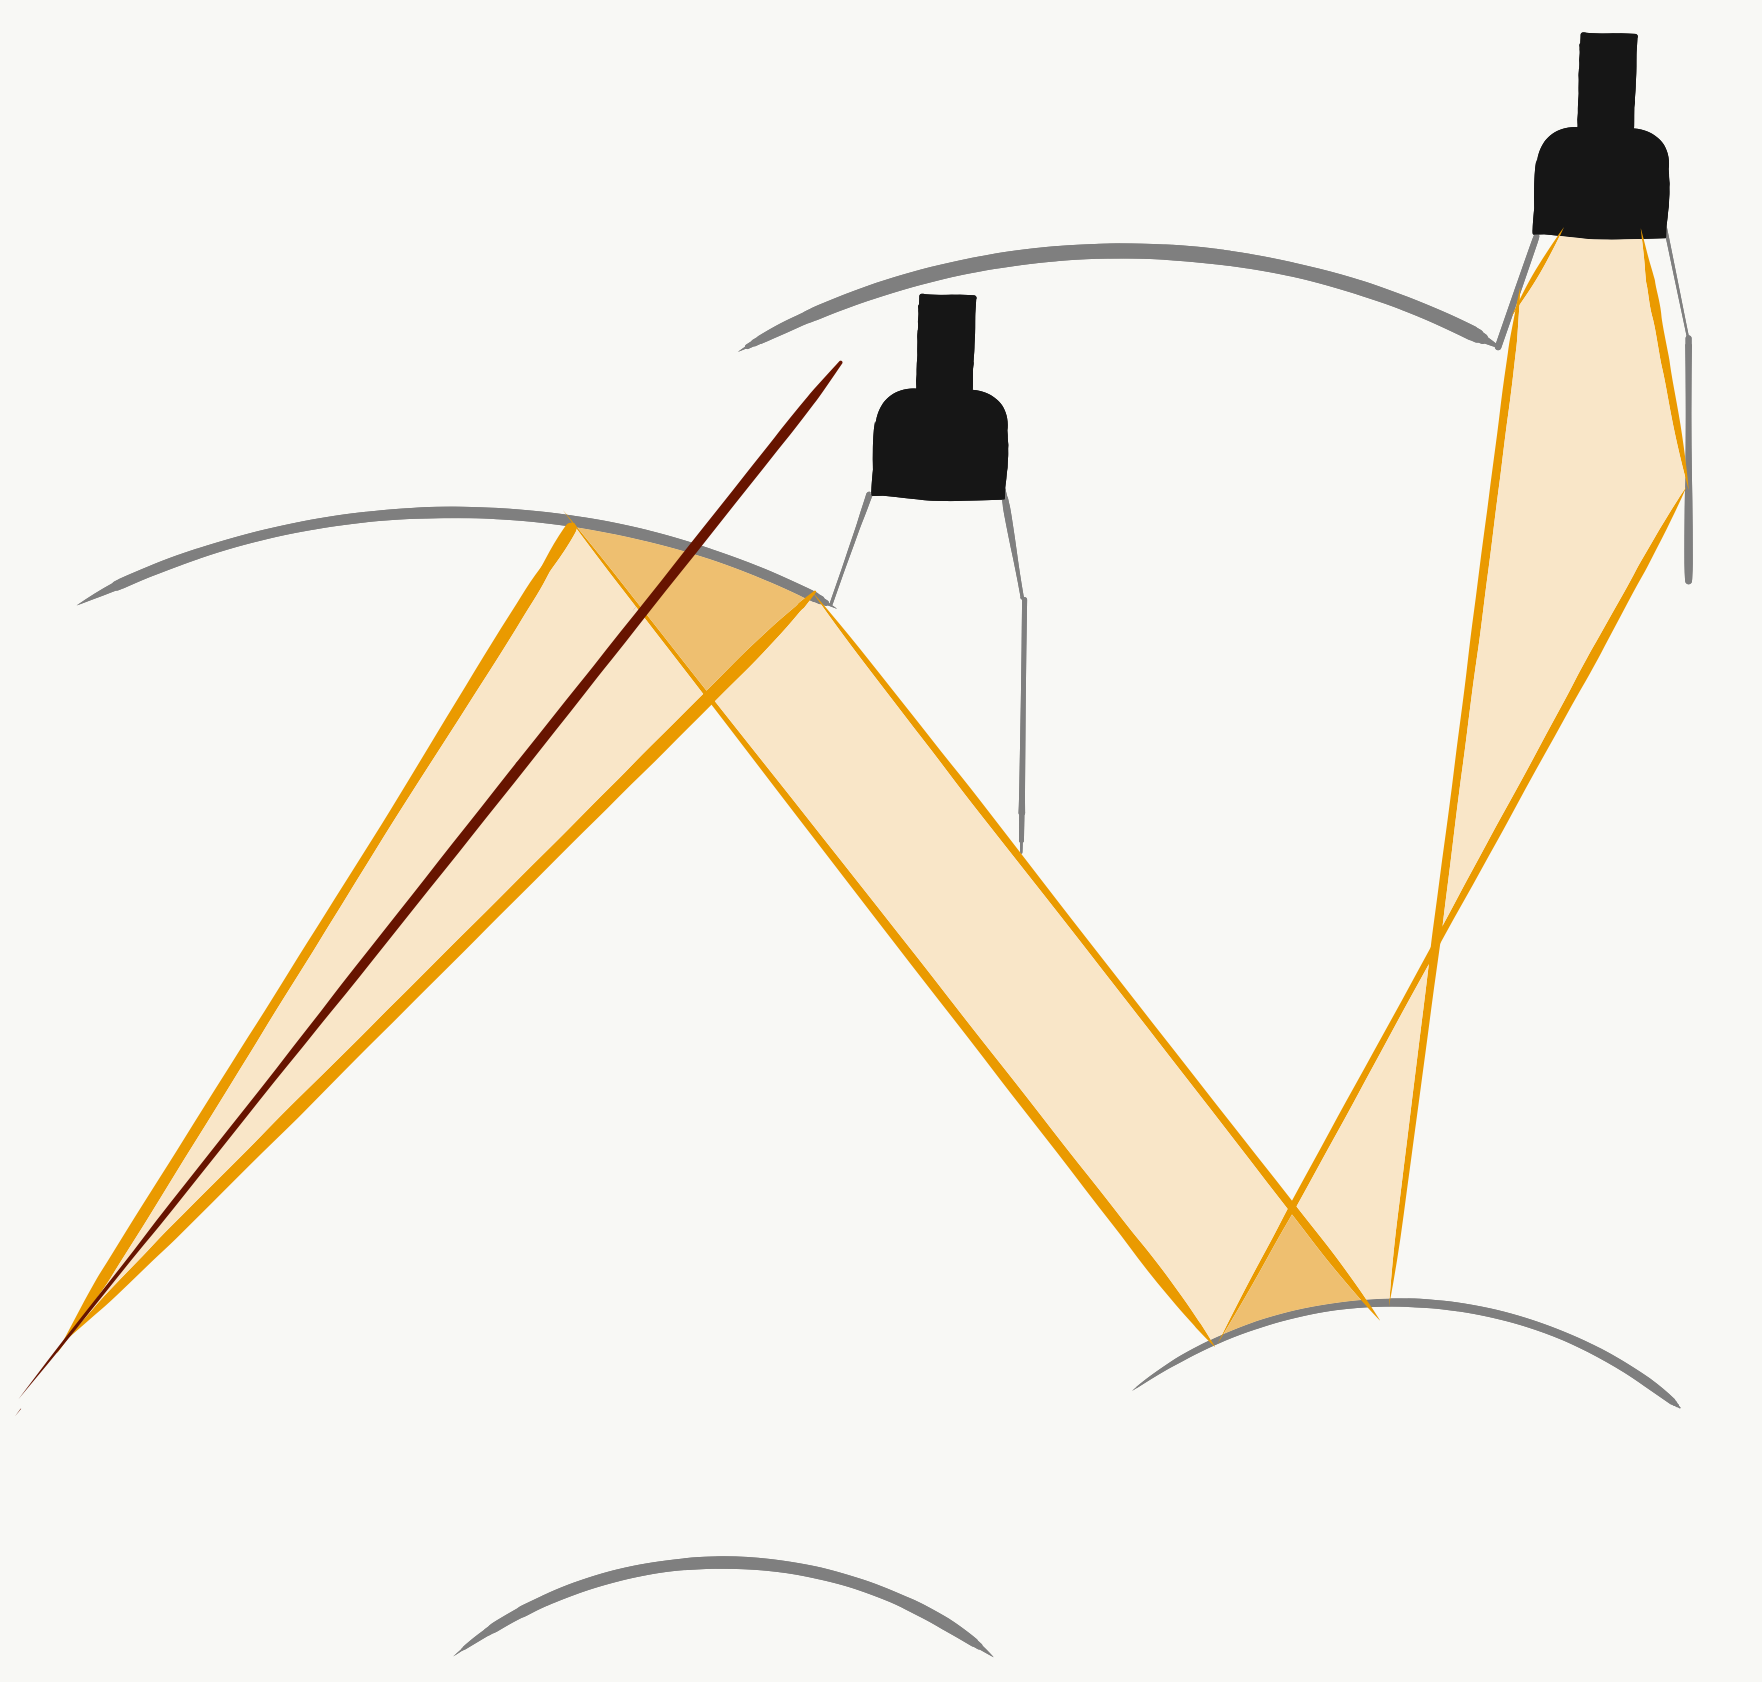
\includegraphics[width=0.99\columnwidth, keepaspectratio]{img/LTCC-event-2.png}
  \caption{Two different simulated LTCC hits for particles passing through the same elliptical mirror. Based on
    particle kinematics, either the PMT in the same segment (top) or a neighboring segment (bottom) is hit.}
  \label{fig:trackmatching}
\end{figure}

